\section{Scaling Data Valuation \& Influence Functions}
\label{sec:method}
In light of these issues, we first design a memory and compute efficient gradient projection algorithm called \method, that leverages the inherent gradient structure in backpropagation (Section~\ref{sec:algorithm}). Then, we provide an intuitive theoretical analysis on why gradient projection approaches work in influence functions (Section~\ref{sec:theory}). Finally, we distill our insights obtained from studying (scalable) influence functions into a new open-source software, called \software, which achieves high compatibility, extensibility, and usability, to facilitate data valuation research  (Section~\ref{sec:software}). In this section, we build our arguments at the granularity of each layer (or module) instead of the whole network for clarity.

\subsection{Algorithm: Memory and Compute Efficient Gradient Projection}
\label{sec:algorithm}
Most layers in neural networks, such as linear and convolutional layers, essentially perform matrix multiplication. Given the input $x_i\in\mathbb{R}^{n_i\times T}$, the output $x_o\in\mathbb{R}^{n_o\times T}$, the weight $W\in\mathbb{R}^{n_o\times n_i}$ for the layer, its forward and backward computations can be written as follows:
\begin{flalign}
\text{\textbf{Forward:}}&&x_o =&\,Wx_i&&\\[-0.1ex]
\text{\textbf{Backward:}}&&\text{vec}(\mathcal{D}W)=\sum_{t=1}^Tx_{i,t}\,\otimes&\, \mathcal{D}x_{o,t}\,,\;\;\mathcal{D}x_i=W^\top\mathcal{D}x_o&&\label{eq:backprop}
\end{flalign}
where $T$ denotes for the sequence dimension in language modeling, $\mathcal{D}$ the derivative with respect to the loss, $\otimes$ the Kronecker product, and $\text{vec}(\cdot)$ the vectorization operation. In Eq.~\eqref{eq:backprop}, we observe that gradient $\text{vec}(\mathcal{D}W)$ obtained during backpropagation is structured as a sum of Kronecker products between forward and backward activations. \method\ leverages this observation to impose an additional Kronecker-product structure on the projection matrix $P$ as follows:% by exploiting the mixed-product property of Kronecker product as follows:
\begin{align}
    P\text{vec}(\mathcal{D}W)\triangleq(P_i\otimes P_o)\text{vec}(\mathcal{D}W)=\sum_{t=1}^T(P_i\otimes P_o)(x_{i,t}\otimes\mathcal{D}x_{o,t})=\sum_{t=1}^T P_ix_{i,t}\otimes P_o\mathcal{D}x_{o,t}\label{eq:logra}
\end{align}
where $P_i\in\mathbb{R}^{k_i\times n_i}$, $P_o\in\mathbb{R}^{k_o\times n_o}$, and $P=P_i\otimes P_o$. In Eq.~\eqref{eq:logra}, \method\ first projects forward and backward activations onto low-dimensional spaces with $P_i$ and $P_o$ respectively, and then reconstructs projected gradient directly from these projected activations. This is in contrast to traditional gradient projection~\cite{park2023trak}, which first computes raw gradient and then projects it onto a low-dimensional space.

Now, we compare memory/compute efficiency of \method\ to that of naive gradient projection, especially under the setting of $n_i\approx n_o\approx\sqrt{n}$ and $k_i\approx k_o\approx\sqrt{k}$. First, both memory/compute costs of per-sample gradient computations reduce from $O(bn)$ to $O(bk)$. Second, both memory/compute costs of gradient projection reduce from $O(bnk)$ to $O(b\sqrt{nk})$. To clearly see this benefit, given the model/projection sizes of 8B/4k, we note that projection matrix sizes are about 1GB and 128TB respectively for \method\ and naive projection. As such, while enjoying general efficiency gains from gradient projection we disscussed in Section~\ref{sec:background}, \method\ further improves the efficiency of per-sample gradient computations significantly at a marginal cost of the additional gradient projection process.


\begin{wrapfigure}{r}{0.26\textwidth}
  \begin{center}
  \vskip -18pt
    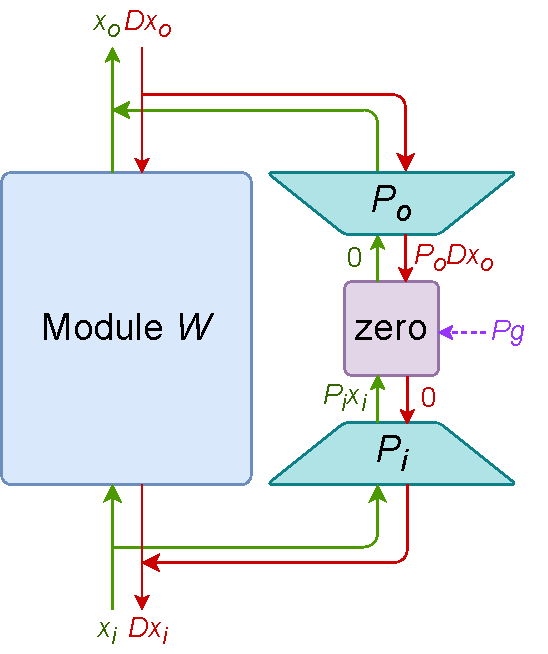
\includegraphics[width=0.26\textwidth]{figures/logra2.pdf}
  \end{center}
  \vskip -8pt
  \caption{\method.}
  \vskip -10pt
  \label{fig:logra}
\end{wrapfigure}

Furthermore, leveraging the fact that projection occurs in the activation space, \method\ can be easily implemented with small add-on layers that are composed of \textit{encoder}, \textit{bottleneck}, and \textit{decoder}, each of which is initialized with $P_i$, zero, and $P_o$ as shown in Figure~\ref{fig:logra}. If we ignore the bottleneck layer, the overall architecture is identical to the popular LoRA architecture \cite{hu2021lora}. While it is intuitive that the roles of encoder and decoder are projecting forward and backward activations respectively, we emphasize two critical roles of the bottleneck layer here. First, its zero initialization ensures that the rest of both forward and backward computations remain unaffected by these add-on layers. Second, per-sample projected gradients can be obtained by simply computing per-sample gradients for the bottleneck layer, using automatic differentiation of an underlying framework without complicated implementation efforts.
%In the next subsection, we propose two initialization strategies for $P_i$ and $P_o$ while discussing the validity low-rank gradient projection approaches to influence functions.

\subsection{Theory: Why Gradient Projection Works in Influence Functions}
\label{sec:theory}
While \method\ can significantly improve scalability of influence functions, an inherent criticism of any gradient projection approach is that information loss from the projection process may render the resulting influence analysis invalid. Unfortunately, theoretical analyses from prior work~\cite{park2023trak,schioppa2022scaling} only discuss the indirect effect of gradient projection on proxy concepts like gradient flow or iHVP variance, which are loosely related to influence functions. To promote trust in the data valuation process, we provide here a mathematical motivation of gradient projection approaches to influence functions. Toward this goal, we interpret a damping term in influence functions that is typically added to ensure the invertibility of the Hessian $H$ as a \textit{spectral gradient sparsification} mechanism. A formal argument and our derivation are respectively provided in Lemma~\ref{eq:lemma} and in Appendix~\ref{sec:derivation}.
\begin{lemma}
\label{eq:lemma}
Let $\{e_1,\cdots,e_n\}$ and $\{\lambda_1,\cdots,\lambda_n\}$ be eigenvectors and eigenvalues of the Hessian $H$. Expressing $g_{tr/te} =\sum_ic_{tr/te,i}\cdot(\sqrt{\lambda_i}e_i)$, the following holds under Assumption~\ref{eq:assumption1}:
\begin{align*}
  \textsc{Influence}(x_{tr}, x_{te}) = g_{te}^\top (H+\lambda I)^{-1}g_{tr} = \sum_{i=1}^n\frac{\lambda_i}{\lambda_i+\lambda}c_{tr,i}c_{te,i}\;\;\text{and}\;\;\mathbb{E}[c_{\cdot,i}^2]\approx 1.  
\end{align*}
\end{lemma}
Lemma~\ref{eq:lemma} shows that a damping term \textit{softly} limits the number of components in influence computations by penalizing contributions from small components. Given the prevalence and practical importance of a damping term in influence functions~\cite{basu2020influence}, we can motivate gradient projection as an alternative way of (hard-)limiting influence computations to components in the projection matrix.
To make \method\ similarly penalize small components, we develop an initialization scheme that exploits the Kronecker-Factored Approximate Curvature (KFAC) algorithm~\cite{martens2015optimizing}.
As a quick overview, KFAC approximates the block-wise Hessian with the Kronecker product of uncentered forward and backward covariances of each layer, respectively denoted with $C_F$ and $C_B$, as $H\approx H_{KFAC} = C_F \otimes C_B$.
Expressing $C_F$ and $C_B$ as $Q_F\Lambda_FQ_F^\top$ and $Q_B\Lambda_BQ_B^\top$ with eigendecomposition, it is easy to show that eigenvectors and eigenvalues of $H_{KFAC}$ are $Q_F\otimes Q_B$ and $\Lambda_F\otimes \Lambda_B$. Consequently, we can approximately discard the smaller components of $H$ by initializing $P_i$ and $P_o$ with $Q_F^{1:k_i}$ and $Q_B^{1:k_o}$, where $Q_\cdot^{1:k}$ is a collection of top-$k$ eigenvectors (similar to performing PCA on forward and backward activations). In Section~\ref{sec:experiments}, we experiment with both PCA and random initialization schemes.

\subsection{Software: Compatibility, Extensibility, and Usability}
\label{sec:software}
Besides algorithmic efficiency, another major bottleneck in the practical adoption of data valuation systems is often the challenge of implementation. In particular, we observe that gradient computation in LLMs, which is a building block for influence functions, typically requires support from other scalability tools like DeepSpeed~\cite{rasley2020deepspeed} or relies on high-level frameworks like HF Transformers~\cite{wolf-etal-2020-transformers}. However, most existing software that can be used for data valuation (\eg,\ Captum~\cite{kokhlikyan2020captum} and TRAK \cite{park2023trak}) is largely incompatible with these tools due to the (too) high level of abstraction in their APIs. 

\begin{wrapfigure}{r}{0.47\textwidth}
\vskip -18pt
\begin{lstlisting}
import logix

# setup
run = logix.init(project, config)
run.setup("stat": "kfac", "save": "grad")
run.watch(model)

# train log & statistic
for batch in train_loader:
  with run(data_id=batch["input_ids"]):
    loss = model(batch)
    loss.backward()
run.finalize()

# test time influence analysis
with run(data_id=tst_batch["input_ids"]):
  loss = model(tst_batch)
  loss.backward()
run.compute_influence_all()
\end{lstlisting}
\vskip -10pt
\caption{Code Example of \software.}
\vskip -11pt
\label{fig:code}
\end{wrapfigure}
%To bridge this gap, we introduce a new data valuation software package, \software, that prioritizes compatibility with other tools in the LLM ecosystem.
Subsequently, we develop a new software package, \software, design of which enables an \textit{easy conversion} of users' existing training code into data valuation code, by promoting compatibility with other tools in the LLM ecosystem.
To this end, we first notice that most influence function algorithms simply require collecting train logs (\eg,\ gradient, activation) and their statistics (\eg,\ covariance). As a result, given arbitrary users' training code, data valuation software only need to intercept these logs, and provide basic primitives to compute various statistics with them. Leveraging this observation, \software\ implements log interceptions and compute primitives using PyTorch hooks. Notably, the use of hooks makes \software\ \textit{compatible} with diverse other tools as hooks can be seamlessly integrated with most PyTorch features (\eg,\ FSDP, autocast, compile). In addition, \software\ is \textit{extensible}, as users can easily define and add custom primitives inside hooks. Finally, \software\ is \textit{easy-to-use} as its context manager automatically handles adding appropriate hooks and primitives to relevant modules with minimal code changes. In Appendix~\ref{sec:logix_appendix}, we provide a more detailed comparison between \software\ and other relevant (interpretability) software, and describe notable optimization techniques (\eg,\ efficient data IO) implemented in it.
Code examples can be found in Figure~\ref{fig:code}, Appendix~\ref{sec:code}, and our project \href{https://github.com/logix-project/logix}{page}.
